\section{Introduction}
% Troubleshooting, but have repair overhead
Troubleshooting algorithms, in general, plan a sequence of actions that are intended to fix an abnormally behaving system. Fixing a system includes repairing faulty components. Such repair actions incur a cost. These costs can be partitioned to two types of repair cost. The first, referred to as the {\em component repair cost}, is the cost of repairing a component. The second, referred to as the {\em repair overhead}, is the cost of preparing the system to perform repair actions (e.g., halting the system may be required), and the cost of testing the system after performing a repair action.

% Thus, batch repair makes sense. Introducing BRP
This paper considers the case where the repair overhead is not negligible and is potentially more expensive than a component repair cost (of a single component). Therefore, it may be more efficient to repair a batch of components in a single repair action. We call the problem of choosing which batch of components to repair the Batch Repair Problem (BRP). BRP is an optimization problem, where the task is to minimize the {\em total repair costs}, which is the sum of the repair overheads and component repair costs incurred by all the repair actions performed until the system is fixed.

% Terminology : fix and repair
Note that in this paper we use the term ``repair'' for a single or a set of components and the term ``fix'' to refer to the entire system.  Thus, {\em repairing} components eventually causes the system to be {\em fixed}, and a system is only fixed if it returned to its nominal behavior.

%\meir {i think we should say something like this explicitly: We consider, in this paper, two kinds of repair costs. The first is the cost of the replaced component. The second is the cost of the system check after repairing some component(s). We assume in this paper that the system check cost is more expensive than the cost of rearing a single component, and therefore it is be more efficient to repair multiple components before operating a system check. }

%Such repair actions incur various costs beyond the cost of repairing the actual components. Such costs can include the overhead of initiating a repairing process, e.g., halting an assembly line, as well as the cost of testing the system after a repair to verify that problem has been fixed. We call these overhead cost the {\em repair overhead}.\footnote{In addition to the repair overhead, one may also consider the cost of the system not being operational~\cite{friedrich1992choosing}.} We study the problem of how to choose which components to repair, so as to minimize the total costs of repairing a system: the repair overhead costs incurred until the system is fixed plus the cost incurred for repairing the individual components.

% Previous work did not try to batch-repair. We need a cost-effective solution that does.
Most previous work assumed that components are repaired one at a time \cite{heckerman1995decision,friedrich1992choosing,Nyberg12,Torta14}. This approach can be wasteful for BRP. For example, if a diagnosis engine infers that multiple faulty components need to be repaired to fix the system, then it would be wasteful to repair these components one at a time -- each repair action incurring its repair overhead. Instead, an efficient BRP algorithm would repair all the faulty components in a single repair action. More generally, we expect an intelligent BRP algorithm to weigh the cost of repairing batches of components as well as the repair overhead.

% Why is BRP hard.
Due to the repair overhead, repairing a single component, even if it is the component most likely to be faulty, can be wasteful. This is especially wasteful in cases where all the found diagnoses consists of multiple faulty components, thus suggesting that repairing a single component would not fix the problem. Alternatively, one may choose to first select to repair the most likely diagnoses, and then repair the set of components in it. This may also be wasteful, especially if there are several diagnoses which have similar likelihood. It might be worthwhile to repair in a single repair action a set of components that ``covers'' more than a single diagnosis. This may reduce the number of repair actions until the system is fixed, thus saving repair overhead costs. However, the component repair costs in such a case can be high, as more components are repaired.


\begin{wrapfigure}{}{4cm}
\begin{center}
  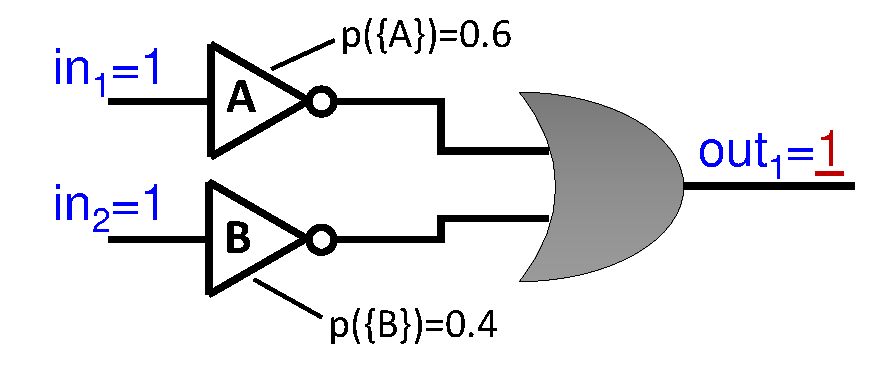
\includegraphics[width=0.5\columnwidth]{simple-example.pdf}
  \caption{An example where repairing components one at a time is wasteful.}
  \label{fig:simple-example}
\end{center}
\end{wrapfigure}
%
%\begin{figure}%
%\centering
%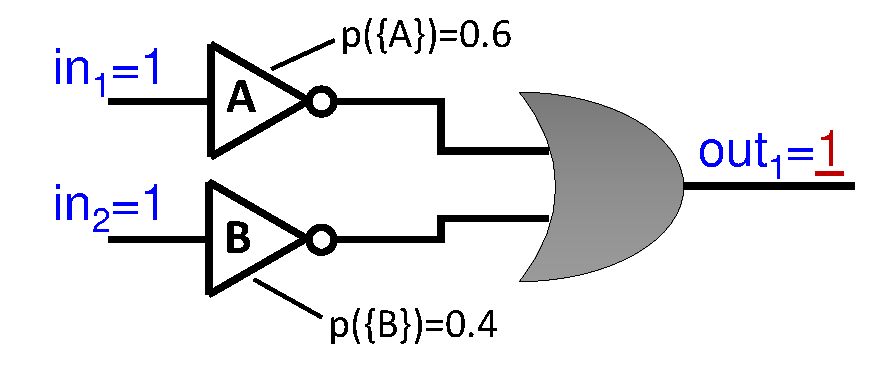
\includegraphics[width=0.6\columnwidth]{simple-example.pdf}%
%\caption{An example where repairing components one at a time is wasteful.}% If $cost_{repair}=10$ and $cost_A=cost_b=1$, the best repair action is to repair $A$ and $B$ together.}%
%\label{fig:simple-example}%
%\end{figure}
%
For example, consider the small system described in Figure~\ref{fig:simple-example}. It is a logical circuit whose output is fault. Assume that the ``OR'' gate is known to be healthy and there are only two possible diagnoses: either $A$ is faulty or $B$ is faulty, where the probability that $A$ and $B$ are faulty is 0.6 and 0.4, respectively. There are three possible repair actions: to repair $A$, to repair $B$, and to repair $A$ and $B$.
Assume the repair overhead costs 10, and repairing a component costs 1. If A is repaired, there is a 0.4 chance that the system would not be fixed and another repair action would be needed (repairing $B$). Thus, the expected total repair cost of repairing $A$ first is 15.4. Similarly, the total repair cost for repairing $B$ first is 17.6. The best option is thus to repair $A$ and $B$ together in a  single repair action, incurring a total repair cost of 12.


%the repair overhead is larger than the cost of repairing a single component. \meir{i do  not understand the last sentence. the reason that repairing all the components is inefficient is due to the high cost of the components and not because the cost of the overhead.}

%Alternatively, one may consider repairing all the components in a single diagnosis, e.g., the most probable diagnosis. This too, however, may be inefficient in cases where the repair overhead is larger than the cost of repairing a single component. \meir{i do  not understand the last sentence. the reason that repairing all the components is inefficient is due to the high cost of the components and not because the cost of the overhead.} For example, consider the system depicted in X \meir{very important to add an example}

%\meir {i think we should say something like this explicitly: We consider, in this paper, two kinds of repair costs. The first is the cost of the replaced component. The second is the cost of the system check after repairing some component(s). We assume in this paper that the system check cost is more expensive than the cost of rearing a single component, and therefore it is be more efficient to repair multiple components before operating a system check. }

% We first show how to optimally do this
We propose two approaches to solve BRP. The first models BRP as a planning under uncertainty problem, where the task is to find a {\em repair policy}, mapping a state of the system to the repair action that minimizes the expected total repair costs. %Specifically, we formalize BRP as a Markov Decision Process (MDP), where the MDP actions are repair actions and the MDP states are the possible states of the system during the repair process. 
This approach combines planning and model-based diagnosis to decide intelligently which sets of components to repair until the problem is fixed. Under some conditions, this approach can return optimal solutions.
The second considers BRP as a combinatorial optimization problem, searching in the space of possible repair actions for the best repair action. We analyze what should the best repair action be and propose several heuristics for choosing the best repair actions in practice.

%Both approaches are unfeasible in large systems, as the number of repair actions would be just too large. We propose a range of possible relaxations, considering only a subset of the possible repair actions, to tradeoff runtime for solution quality.
%\meir{We first propose an optimal algorithms by modeling the planning problem as Markov Decision Process (MDP). The optimal algorithm guarantees repairing the system with minimal cost but its runtime is exponential. We propose then some relaxations to reduce the exponential runtime of the MBD and the MDP.}

%\meir{i do not know how, but we should prepare the reader in the abstract and here that this is a theoretical work and although it is important. Roni: Added the paragraph below}

The contributions of this work are theoretical. We model the BRP problem formally, discuss how it relates to other troubleshooting problems and propose two approaches to solve it. Also, we propose a range of possible relaxations, applicable to both approaches, where only a subset of the possible repair actions are considered. These relaxations can allow scaling to larger systems, trading runtime for solution quality.

%This lays the foundation for future work that would examine the effectiveness of the range of suboptimal solvers we propose in practical domains.


\section{Problem Definition}
% Classical input
A classical MBD input $\langle SD,COMPS,OBS \rangle$ is assumed, where SD is a model of the system, COMPS is the of system components, and OBS is the observed behavior of the system. %Every component can be either healthy or faulty.\footnote{Behavior modes are discussed later in the paper.} The assumption that a component $C_i\in COMPS$ is healthy is represented by the health predicate $h(C_i)$.
Every component can be either normal or abnormal. %\footnote{Behavior modes are discussed later in the paper.}
The assumption that a component $C_i\in COMPS$ is abnormal is represented by the abnormal predicate $AB(C_i)$.

% When the problem happens
\noindent A {\em batch repair problem} (BRP) arises when the assumption that all components are normal is not consistent with the system description and observations. Formally,
\[ SD \wedge OBS \wedge \bigwedge_{C_i\in COMPS} \neg AB(C_i) ~~~ \text{is not consistent} \]
\noindent In such a case, at least one component must be repaired.

\begin{definition}[Repair Action]
A repair action can be applied to any subset of components and results in these components becoming normal. Applying a repair action to a set of components $C'$ is denoted by Repair($C'$).
\label{def:repairAction}
\end{definition}
Definition~\ref{def:repairAction} assumes that repair actions always succeed, i.e., a component is normal after it is repaired. %[Roni: TODO: discuss how to relax this assumption later in the paper.]

% What happens after a repair action
After a repair action, the system is tested to check if it has been fixed.
We assume that the system inputs in this test are the same as in the original observations ($OBS$). The observed system outputs are then compared to the expected system outputs of a healthy system. Thus, the result of a repair action is either that the system is fixed, or a new observation that may help choosing future repair actions.

% Repairing incurs a cost
Repairing a set of components incurs a cost, composed of a repair overhead and component repair costs. The repair overhead is denoted by $cost_{repair}$, and the component repair cost of a component $C_i\in COMPS$ is denoted by $cost_{C_i}$.

%The repair overhead correspond to the system costs involved in initiating a repair action, e.g., stopping an assembly line to take out the components to be repaired, as well as the cost of testing the system's behavior after the repair action was performed. The component repair cost $cost_{C_i}$ correspond to the actual cost of repairing $C_i$, e.g., the cost of replacing the faulty parts of $C_i$.

%\meir{the notations are confusing. you have two types of costs so name both cost. the overhead can be $cost_{ovrhd}$ and the cost of component $cost_{C_i}$ Roni: modified as you said +-}

\begin{definition}[Repair Costs]
Applying a repair action Repair($C$) incurs a cost:
\[ cost(Repair(C)) = cost_{repair} + \sum_{C_i\in C} cost_{C_i} \]
\end{definition}
We assume that all repair costs are positive and non-zero, i.e., $cost_{repair}>0$ and $cost_{C_i}>0$ for every component $C_i \in COMPS$. As defined earlier, the task in BRP is to fix a system with minimum total repair cost.

%We denote by {\em total repair cost} this sum of repair costs incurred until the system is healthy,
%and call the problem of minimizing the total repair cost the Batch Repair Problem (BRP).

As shown in Figure~\ref{fig:simple-example}, an efficient BRP solver should consider the possibility of repairing a set of components in a single repair action. Thus, the potential number of repair actions is %exponential in the number of components, in particular the power set of the components 
$2^{|COMPS|}$. Therefore, from a complexity point of view BRP is an extremely hard problem.


%BRP differs from other troubleshooting problems in the assumption that $C_{repair}>0$. \meir{i do not agree. f.i. heckermann assumed this. the different is the multiple component repair.} This assumption entails that an algorithm for solving BRP should consider the possibility of repairing a set of components in a single repair action. This causes the potential number of repair actions to be exponential in the number of components, in particular the power set of the components $2^{|COMPS|}$. Thus, from a complexity point of view BRP is an extremely hard problem.

%[[Roni: is the paragraph above redundant?]] \meir{no it is ok}
%\meir{i think it is important to say that this problem becomes interesting once we have 1. multiple faults 2. the cost of repair >> cost of a single component. Roni: it is enough for $C_{repair}$ to only be not zero. Regarding multiple faults, that seems related to the solution approach and not the problem def. So I added the paragraph above in an attempt to address your point - I hope it is Ok.}